\section{Métodos de programación entera}

\subsection{Relajación Lineal}

\subsection{Cotas superiores e inferiores}

\subsection{Brecha de optimalidad}

\subsection{Método de ramificación y acotamiento, Branch and Bound.}

\subsubsection{Árbol de búsqueda}

\subsubsection{Estrategias de ramificación}

\subsection{Planos cortantes}

\subsection{Criterios de terminación}

\subsection{Ejercicios}

\subsubsection{Ejercicio 5.1}
% Fuente: Auxiliar 8, «Árbol de Branch and Bound».
Suponga que para 
\[
\max \{c^T x : Ax = b, x \geq 0, x \in \mathbb{Z}^n \}
\]
se obtiene el árbol de Branch and Bound de la Figura~\ref{ex:5:1:fig:arbol}. Responda las siguientes preguntas:

\begin{enumerate}
    \item Si ejecutamos B\&B con un \textit{gap} relativo de 10\% y una cota inferior inicial de $-\infty$, ¿es posible terminar después de explorar sólo cuatro nodos? Si es así, ¿cuáles serían las hojas sin explorar?
    \item Si ejecutamos B\&B, y exploramos el nodo 4 antes del nodo 7, ¿sería posible que el nodo 12 sea explorado en algún momento posterior por el algoritmo? Justifique.
    \item Usando sólo el árbol mostrado en la figura, ¿es posible encontrar la solución óptima del problema? Justifique.
    \item ¿Es posible que el conjunto de nodos \textbf{5, 10, 11, 7} sean las hojas del algoritmo de B\&B? Justifique.
    \item ¿Es posible que el conjunto de nodos \textbf{2, 6, 12, 13} sean las hojas del algoritmo de B\&B? Justifique.
\end{enumerate}

\begin{figure}
    \centering
    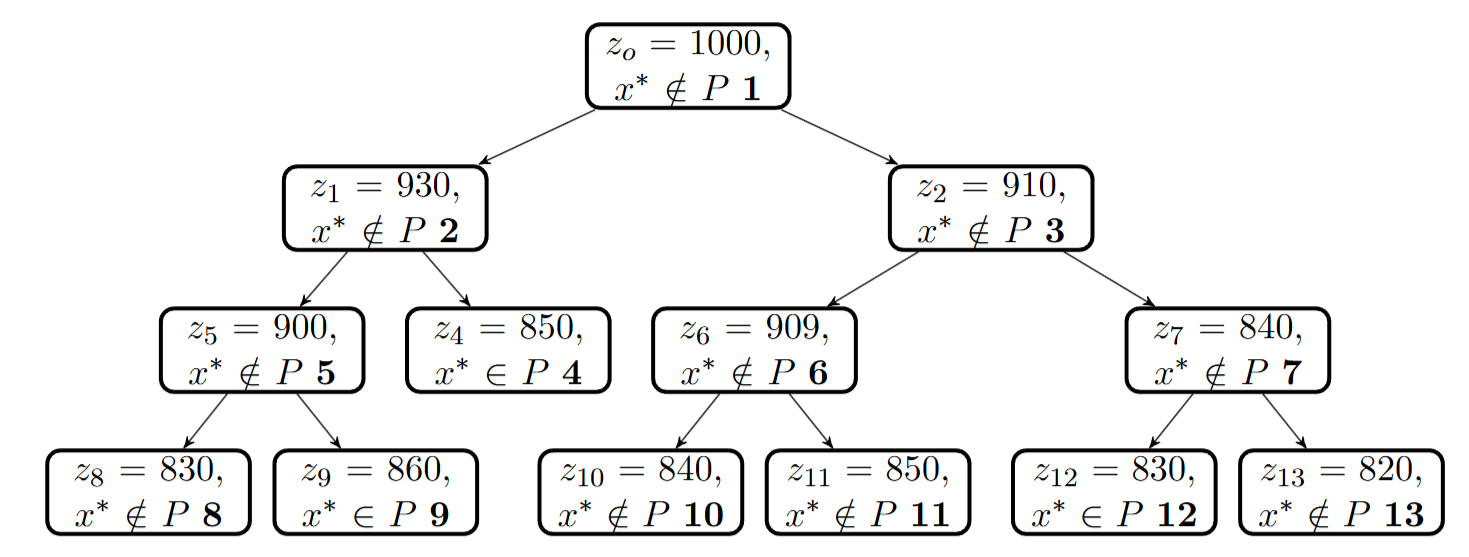
\includegraphics[width=1\linewidth]{img/ejercicios/Capitulo-5/ejercicio_5_1_arbol.png}
    \caption{Árbol de Branch and Bound}
    \label{ex:5:1:fig:arbol}
\end{figure}


\subsubsection{Ejercicio 5.2}
% Fuente: Auxiliar 8, «Métodos de programación entera».
Considere el siguiente problema de programación entera:
\[
\begin{aligned}
\max\quad & x_{1} \;+\; 2\,x_{2} \\[0.5em]
\text{sujeto a}\quad 
& -\,3\,x_{1} \;+\; 4\,x_{2} \;\le 4\\
& 3\,x_{1} \;+\; 2\,x_{2} \;\le 11\\
& 2\,x_{1} \;-\; x_{2} \;\le 5\\
& x_{1},\,x_{2} \;\ge 0,\quad x_{1},\,x_{2} \in \mathbb{Z}.
\end{aligned}
\]
Usar un gráfico para responder las siguientes preguntas:

\begin{enumerate}
  \item[(a)] ¿Cuál es el costo óptimo de la relajación lineal? ¿Y cuál es el costo óptimo del problema de programación entera?
  \item[(b)] ¿Cuál es la envoltura convexa del conjunto de todas las soluciones enteras factibles?
  \item[(c)] Ilustrar cómo funciona el algoritmo de planos de corte de Gomory. Realizar el primer corte.
  \item[(d)] Resolver el problema mediante \emph{branch \& bound}, resolviendo gráficamente las relajaciones.
  \item[(e)] Suponga que se dualiza la restricción \( -\,3\,x_{1} + 4\,x_{2} \le 4 \). ¿Cuál es el valor óptimo \(Z_{D}\) del dual lagrangeano? ¿Cómo cambia el valor de $Z_D$ si se dualiza la restricción \( 2\,x_{1} - x_{2} \le 5 \)? 
\end{enumerate}


\subsubsection{Ejercicio 5.3}
% Fuente: Auxiliar 10, «Repaso de programación entera — Branch and Bound».
En la figura~\ref{ex:5:3:fig:bnb} se observa el árbol con las iteraciones del algoritmo Branch and Bound para un problema de optimización. Cada nodo representa un subproblema y contiene la información del valor objetivo de ese subproblema y si es que la solución encontrada es entera (E), fraccional (NE) o infactible. Note que la etiqueta del problema $P_3$ no está determinada. Responda las siguientes preguntas:

\begin{enumerate}
    \item Suponga que la solución encontrada en $P_5$ es fraccional (NE) y responda cada caso: ¿Este es un problema de maximización o minimización? ¿Qué nodos ramificaría el algoritmo? ¿Qué cota tiene la función objetivo hasta este punto?
    \item ¿Cómo cambian sus respuestas si la solución del problema $P_5$ fuese entera?
\end{enumerate}

\begin{figure}
    \centering
    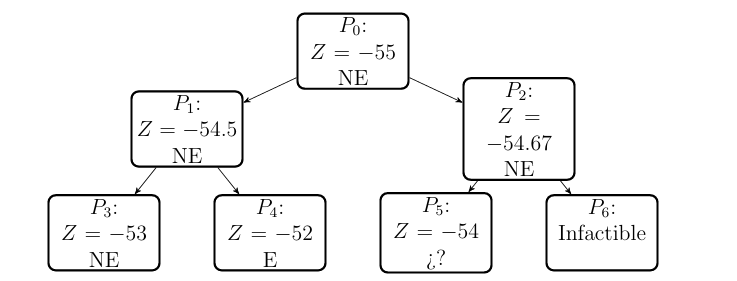
\includegraphics[width=1\linewidth]{img/ejercicios/Capitulo-5/ejercicio_5_3_byb.png}
    \caption{Árbol de Branch and Bound.}
    \label{ex:5:3:fig:bnb}
\end{figure}


\subsubsection{Ejercicio 5.4}
% Fuente: Auxiliar 10, «Repaso de programación entera — Cortes de Gomory».
Considere el siguiente problema de optimización entera:
\[
\begin{aligned}
(P)\quad \min\;& -3x_{1} + 2x_{2}\\
\text{s.a.}\quad
&7x_{1} + 2x_{2} \;\le\; 8,\\
&x_{1} + 2x_{2} \;\le\; 7,\\
&x_{1},\,x_{2}\;\in\;\mathbb{Z}_{\ge0}.
\end{aligned}
\]

\begin{enumerate}
  \item Resuelva gráficamente la relajación lineal de este problema. También muestre la envolvente convexa de los puntos factibles.
  \item Realice una iteración del algoritmo de cortes de Gomory. Discuta gráficamente la optimalidad de la nueva solución encontrada.
\end{enumerate}


\subsubsection{Ejercicio 5.5}
% Fuente: Control 2, Pregunta 1.
El operador de una planta industrial quiere instalar dos tipos de alimentadores
eléctricos para maximizar el número de cargas críticas en hora punta:

\begin{itemize}[nosep]
  \item $x_1$: Alimentadores de distribución tipo A --- energizan $5$ cargas cada uno, demandan $6$\,A de la protección termomagnética principal y ocupan $1$ módulo en el tablero de distribución.
  \item $x_2$: Alimentadores de distribución Tipo B --- energizan $4$ cargas cada uno, demandan $4$\,A de la protección termomagnética principal y ocupan $2$ módulos en el tablero de distribución.
\end{itemize}

La protección termomagnética principal soporta un máximo de $24$\,A y el tablero de distribución solo dispone de $6$ módulos de espacio libre.
 
\begin{enumerate}[label=(\alph*)]
  \item Formule el problema de programación entera. Dibuje la envoltura convexa de las soluciones factibles y encuentre el valor
  óptimo del problema lineal relajado.
  
  \item Proponga un corte o cortes sobre el conjunto factible de modo que el óptimo del problema relajado coincida con el óptimo entero y obtenga el óptimo del problema de forma gráfica.
  
  \textit{No considere (b) para los siguientes incisos}
        
  \item Aplique el primer plano de corte de Gomory sobre el problema original. Muestre y explique cómo afecta al conjunto factible.
  
  \item Resuelva mediante Branch \& Bound (B\&B) usando búsqueda en amplitud. Dibuje el
   árbol de decisiones, indicando en cada nodo la solución de la relajación lineal,
   identifique cada hoja y justifique por qué no se ramifica.
  \item ¿Qué tolerancia de \emph{gap} de optimalidad es necesaria  para que el algoritmo B\&B termine analizando solo $3$ problemas (incluyendo la relajación original), usando búsqueda en amplitud? Analice su respuesta a partir del \textit{trade off} entre un mayor \textit{gap} con una respuesta más precisa.
\end{enumerate}


\subsubsection{Ejercicio 5.6}
% Fuente: Control 2, Pregunta 3, ítems 3–4.
Indique si las siguientes afirmaciones son falsas o verdaderas. En caso de ser verdadera, debe proveer una demostración; en caso contrario, debe dar un contraejemplo.  
\begin{enumerate}
\item Si un programa lineal entero tiene dos soluciones óptimas distintas, entonces tiene infinitas soluciones óptimas. 
\item Sean $P_1$ y $P_2$ las regiones factibles de dos relajaciones de un programa lineal entero de minimización, tales que $P_1 \subseteq P_2$. Si $x^* \in \mathbb{Z}^n$ es una solución óptima del problema entero, con valor óptimo $c^\top x^*$, entonces
$c^\top x^* \geq \min_{x \in P_1} c^\top x \geq \min_{x \in P_2} c^\top x$.
\end{enumerate}


\subsection{Resoluciones}

\subsubsection{Resolución 5.1}
% Fuente: Pauta del Auxiliar 8, «Árbol de Branch and Bound».
Denotemos $z^*$ el incumbente y se entenderá un nodo hoja como uno que no será ramificado (terminal).

\begin{enumerate}
    \item El gap relativo se define como \(\%\text{gap} = \frac{UB - LB}{LB}\), en este caso \(\%\text{gap} = \frac{z^* - LB}{LB}\). De esta forma sí es posible terminar después de explorar 4 nodos, para esto se exploran los nodos \textbf{1, 2, 3} y \textbf{4} y se llega a un \(\%\text{gap} = \frac{930 - 850}{850} = 9.41\% < 10\%\). De esta forma se dejan sin explorar las hojas \textbf{5, 6} y \textbf{7}.
    
    \item No, ya que el incumbente sería al menos 850 (\(z_4 = 850\) y es entero), de esta forma el nodo \textbf{7} no se seguirá ramificando (\(840 = z_7 < z^*\)).
    
    \item Sí, el valor óptimo es \(z = 860\) y se encuentra en el nodo \textbf{9}. Notar que en las demás hojas la función objetivo es menor a este valor.
    
    \item No, de haberse explorado antes el nodo \textbf{4} se tendría \(z^* = 850\), y los nodos \textbf{10, 11, 7} al tener funciones objetivo menores o iguales, efectivamente podrían ser hojas. Sin embargo, no hay manera de que el nodo \textbf{5} sea hoja, ya que no hay solución entera que supere su valor.
    
    \item No, de manera análoga al caso anterior, no hay posibilidad de que los nodos \textbf{2} y \textbf{6} sean hojas.
\end{enumerate}


\subsubsection{Resolución 5.2}
% Fuente: Pauta del Auxiliar 8, «Métodos de programación entera».
\begin{enumerate}
  \item[(a)] Gráficando el conjunto factible se tiene:
  \begin{figure}
      \centering
      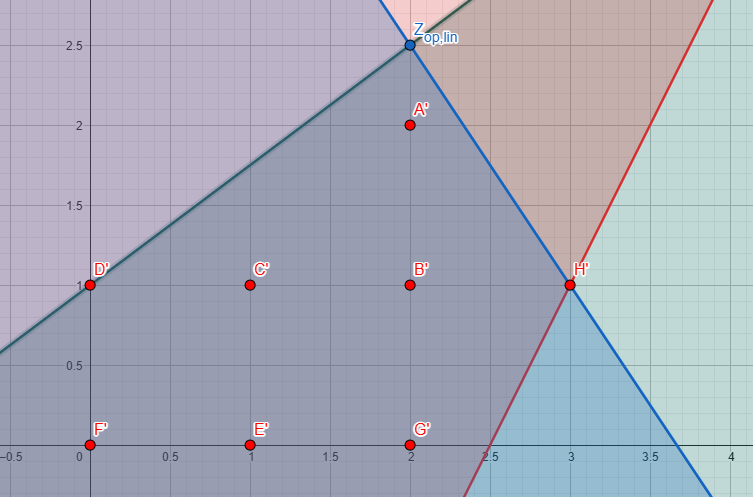
\includegraphics[width=0.7\linewidth]{img/ejercicios/Capitulo-5/ejercicio_5_2_metodos_programacion_entera.png}
      \caption{Conjunto factible Pregunta 3.}
      \label{ex:5:2:fig:conjunto-factible}
  \end{figure}
  La solución de la relajación lineal y del problema original son:
  \[
    z_{\text{LP}} = 7,\quad\text{en }(x_{1},x_{2})=(2,2.5),
    \qquad
    z_{\text{IP}} = 6,\quad\text{en }(x_{1},x_{2})=(2,2).
  \]
  
  \item[(b)] Si se enumeran las soluciones enteras factibles:
  \[
  \{(0,0),(1,0),(2,0),(0,1),(1,1),(2,1),(2,2),(3,1)\}
  \]
  su envoltura convexa es el polígono de vértices
  \[
    \{(0,0),\quad(2,0),\quad(3,1),\quad(2,2),\quad(0,1).\}
  \]
  Es decir,
  \[
    \mathrm{conv}\bigl\{(0,0),(2,0),(3,1),(2,2),(0,1)\bigr\}.
  \]
  Las siguientes rectas producen la envoltura convexa:
  \begin{align*}
      & x_1\geq0\\
      & x_2 \geq 0\\
      & x_2 \geq x_1 -2 \\
      & x_2 \leq 0.5 x_1 +1\\
      & x_2 \leq -x_1 +4
  \end{align*}
  
  \item[(c)] Las matrices del problema relajado en formulación estándar son:
  \[
  A=\begin{pmatrix}
    -3 & 4 &1 & 0 & 0 \\
    3 & 2 & 0 &1&0 \\
    2 & -1&0&0&1
\end{pmatrix}, \quad b= \begin{pmatrix}
    4 \\
    11 \\
    5 
\end{pmatrix}, \quad B=
    \begin{pmatrix}
        -3 & 4 &0  \\
        3 & 2 & 0  \\
        2 & -1&1
    \end{pmatrix}
  \]
  El óptimo de la relajación lineal es $(2,2.5,0,0,5.3)$, luego se realiza el corte sobre $x_2$:
  \begin{equation}
      x_2 + \lfloor\overline{a_{23}}\rfloor \cdot s_1+\lfloor\overline{a_{24}}\rfloor \cdot s_2 \leq \lfloor\overline{a_{20}}\rfloor
  \end{equation}
  donde:
  \begin{align}
     & \overline{a_{23}}=\left(B^{-1}\begin{pmatrix}
          1  \\ 0 \\ 0
      \end{pmatrix} \right)_2 =\frac{1}{6} \\
    & \overline{a_{23}}=\left(B^{-1}\begin{pmatrix}
          0  \\ 1 \\ 0
    \end{pmatrix} \right)_2 =\frac{1}{6} \\
    & \overline{a_{23}}=\left(B^{-1}b \right)_2 =2.5
  \end{align}
De modo que el nuevo corte es:
\begin{equation}
    x_2 \leq 2
\end{equation}
  
  \item[(d)] Comenzamos con $L=-\infty$, donde L corresponde a la mejor corta inferior al ser un problema de maximización.
  
  El nodo raíz corresponde a resolver la relajación lineal del problema original, luego $(x_1, x_2)=(2,2.5)$, donde $z=7$. Dado que no tiene solución entera, se selecciona $x_2$ para particionar el conjunto factible. No se actualiza la cota ($L=-\infty$).

  Los subproblemas generados son:

\begin{equation}
\begin{aligned}
(P2)\quad \min\;& -x_1 \;-\; 2x_2 \\
\text{s.a.}\;& -3x_{1} + 4x_{2} \le 4,\\
& 3x_{1} + 2x_{2} \le 11,\\
& 2x_{1} - x_{2} \le 5,\\
& x_{2} \le 2,\\
& x_{i} \ge 0,\quad i\in\{1,2\}.
\end{aligned}
\end{equation}

\begin{equation}
\begin{aligned}
(P3)\quad \min\;& -x_1 \;-\; 2x_2 \\
\text{s.a.}\;& -3x_{1} + 4x_{2} \le 4,\\
& 3x_{1} + 2x_{2} \le 11,\\
& 2x_{1} - x_{2} \le 5,\\
& x_{2} \ge 3,\\
& x_{i} \ge 0,\quad i\in\{1,2\}.
\end{aligned}
\end{equation}

Dado que el problema $(P3)$ es infactible, se descarta. El problema $(P2)$ alcanza el óptimo en:
\begin{equation}
    x=\left(\frac{7}{3},2\right), \quad z= \frac{19}{3}
\end{equation}
    
Como la solución es no entera, se elige $x_1$ para particionar el conjunto. Aún no hay solución entera, por lo que $L=-\infty$.

Los subproblemas generados a partir de $(P2)$ son:

\begin{equation}
\begin{aligned}
(P4)\quad \min\;& -x_1 \;-\; 2x_2\\
\text{s.a.}\;& -3x_{1} + 4x_{2} \le 4,\\
& 3x_{1} + 2x_{2} \le 11,\\
& 2x_{1} - x_{2} \le 5,\\
& x_{2} \le 2,\\
& x_{1} \le 2,\\
& x_{i} \ge 0,\quad i\in\{1,2\}.
\end{aligned}
\end{equation}

\begin{equation*}
\begin{aligned}
(P5)\quad \min\;& -x_1 \;-\; 2x_2\\
\text{s.a.}\;& -3x_{1} + 4x_{2} \le 4,\\
& 3x_{1} + 2x_{2} \le 11,\\
& 2x_{1} - x_{2} \le 5,\\
& x_{2} \le 2,\\
& x_{1} \ge 3,\\
& x_{i} \ge 0,\quad i\in\{1,2\}.
\end{aligned}
\end{equation*}

La solución de $(P4)$ es:
\begin{equation}
    x=(2,2), \quad z=6
\end{equation}
 Como la solución es entera, se actualiza la cota $L=6$.

 La solución de $(P5)$ es:
 \begin{equation}
     x=(3,1), \quad z= 5
 \end{equation}
 Dado que $z\le L$, se descarta $(P5)$ y la cota superior se mantiene en $L=6$.

 Finalmente, tras explorar todos los nodos, la mejor solución entera es:
 \begin{equation}
    x=(2,2), \quad z=6
\end{equation}
la cual corresponde a la solución del problema original.
  
  \item[(e)] Dado que se está maximizando, se obtendrán cotas superiores. Al relajar dicha restricción con multiplicador \(p\ge0\), el lagrangiano queda:
    \[
      Z(p)
      = \max_{x_{1},x_{2}}
      \Bigl\{\,x_{1} + 2x_{2}
      \;+\; p\,(4 + 3x_{1} - 4x_{2})\Bigr\}
      \quad\text{s.a.}\quad
      \begin{cases}
        3\,x_{1} + 2\,x_{2} \;\le\; 11,\\
        2\,x_{1} - x_{2} \;\le\; 5,\\
        x_{1},x_{2}\ge0,\;x_{1},x_{2}\in\mathbb{Z}.
      \end{cases}
    \]
    Los puntos factibles \((x_{1},x_{2})\) (ignorando la restricción dualizada) generan las siguientes funciones candidatas
    \(\displaystyle\overline{Z}(p)=x_{1}+2x_{2}+p\,(4+3x_{1}-4x_{2})\):

    \[
      \begin{array}{cc|c}
        \hline
        x_{1} & x_{2} & \overline{Z}(p) \\ \hline
        0 & 0 & 4\,p              \\
        0 & 1 & 2                  \\
        0 & 2 & 4 - 4\,p          \\
        0 & 3 & 6 - 8\,p          \\
        0 & 4 & 8 -12\,p          \\
        0 & 5 & 10-16\,p          \\[4pt]
        1 & 0 & 1 + 7\,p          \\
        1 & 1 & 3 + 3\,p          \\
        1 & 2 & 5 -   p          \\
        1 & 3 & 7 - 5\,p          \\
        1 & 4 & 9 - 9\,p          \\[4pt]
        2 & 0 & 2 +10\,p          \\
        2 & 1 & 4 + 6\,p          \\
        2 & 2 & 6 + 2\,p          \\[4pt]
        3 & 1 & 5 + 9\,p          \\
        \hline
      \end{array}
    \]

    A partir de aquí se toma el envolvente superior de estas rectas para obtener
    \(\;Z(p)=\max_{i,j}\overline{Z}(p)\;\) y luego
    \(\displaystyle Z_{D}=\min_{p\ge0}Z(p)\).

Tomando las funciones candidatas \(\overline{Z}(p)=x_{1}+2x_{2}+p(4+3x_{1}-4x_{2})\)
    en cada punto factible y construyendo el envolvente superior, resulta:
    \[
      Z(p)
      = \max_{(i,j)}\overline{Z}(p)
      = 
      \begin{cases}
        10 - 16\,p, & 0 \le p \le \tfrac17,\\[0.3em]
        9 - 9\,p,   & \tfrac17 \le p \le \tfrac29,\\[0.3em]
        5 + 9\,p,   & \tfrac29 \le p \le 3,\\[0.3em]
        2 +10\,p,   & p \ge 3.
      \end{cases}
    \]
    La mejor cota dual se halla en la intersección de la recta $9+9p$ y $5+9p$:
    \[
      \min_{p\ge0}Z(p)
      \;\Longrightarrow\;
      p^* = \tfrac29,
      \quad Z_{D} = Z\bigl(\tfrac29\bigr) = 7.
    \]

Ahora, al relajar la restricción
    \[
      2x_{1} - x_{2} \le 5
    \]
    con lagrangiano
    \[
      Z(q)
      = \max_{x_{1},x_{2}}
      \Bigl\{\,x_{1} + 2x_{2}
      \;+\; q\,(5 - 2x_{1} + x_{2})\Bigr\}
      \quad\text{s.a.}\quad
      \begin{cases}
        -3x_{1} + 4x_{2} \;\le\; 4,\\
        3x_{1} + 2x_{2} \;\le\; 11,\\
        x_{1},x_{2}\ge0,\;x_{1},x_{2}\in\mathbb{Z}.
      \end{cases}
    \]

    Los puntos factibles \((x_{1},x_{2})\) (ignorando la restricción dualizada) generan las siguientes funciones candidatas:

    \[
      \begin{array}{cc|c}
      \hline
      x_{1} & x_{2} & \overline{Z}(q) \\ \hline
      0 & 0 & 0 + 5q \\
      0 & 1 &  2 + 6q \\
      1 & 0 & 1 + 3q \\
      1 & 1 & 3 + 4q \\
      2 & 0 & 2 + 1q \\
      2 & 1 & 4 + 2q \\
      2 & 2 & 6 + 3q \\
      3 & 0 & 3 - 1q \\
      3 & 1 & 5 + 0q \\ \hline
      \end{array}
    \]

    El valor dual es el envolvente superior de estas rectas:
    \[
      Z(q)
      =
      \begin{cases}
        6 + 3q, & 0 \le q \le \tfrac{4}{3},\\[0.3em]
        2 + 6q, & q \ge \tfrac{4}{3}.
      \end{cases}
    \]
    Como ambas ramas tienen pendiente positiva, el mínimo sobre \(q\ge0\) se logra en
    \[
      q^* = 0,
      \qquad
      Z_{D} = Z(0) = 6.
    \]
\end{enumerate}


\subsubsection{Resolución 5.3}
% Fuente: Pauta del Auxiliar 10, «Repaso de programación entera — Branch and Bound».
\begin{enumerate}
  \item Recordar que al agregar restricciones la solución va empeorando al reducir su región factible. Como en este caso la solución aumenta (es menos negativa), se concluye que se está minimizando. El algoritmo ramificaría los nodos \(P_3\) y \(P_5\) ya que son los únicos que pueden seguir dando una mejor solución. En este caso la cota superior (UB) es el \emph{incumbente} \(=-52\) y la cota inferior viene dada por el nodo \(P_5\) (en el mejor de los casos el óptimo podría ser \(-54\)).
  \item Si la solución de \(P_5\) fuese entera, el algoritmo no sigue ramificando ya que el óptimo se encuentra en ese nodo y ambas cotas coinciden (\(\mathrm{UP} = \mathrm{LB} = -54\)).
\end{enumerate}


\subsubsection{Resolución 5.4}
% Fuente: Pauta del Auxiliar 10, «Repaso de programación entera — Cortes de Gomory».
{\color{MidnightBlue}
\begin{enumerate}
  \item
\begin{figure}
    \centering
    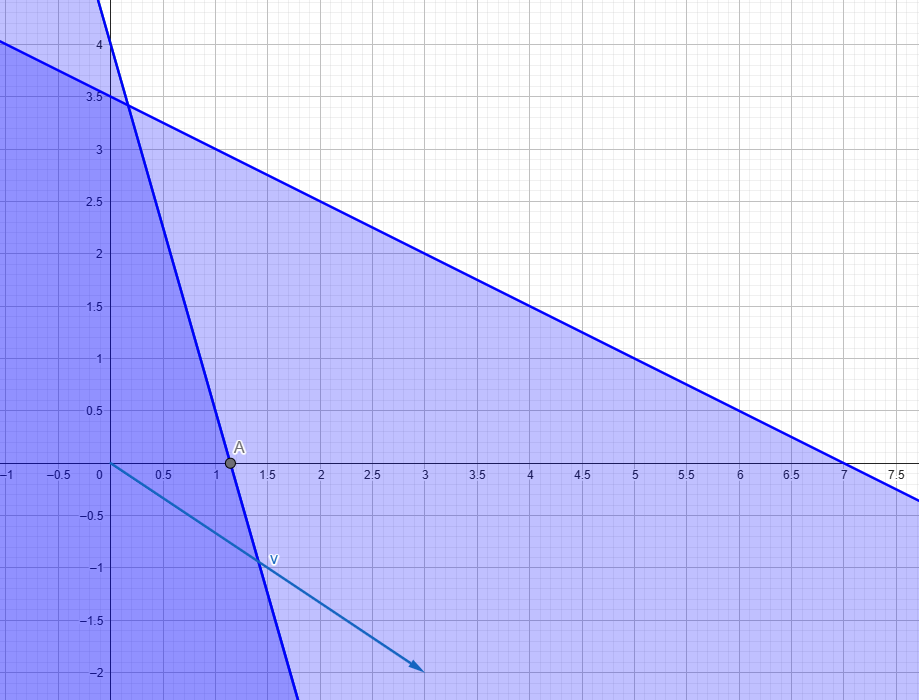
\includegraphics[width=0.8\linewidth]{img/ejercicios/Capitulo-5/ejercicio_5_4_solucion_gomory.png}
    \caption{Solución relajación lineal}
    \label{ex:5:4:fig:relajacion}
\end{figure}
    
El óptimo de la relajación se obtiene en
\[
(x_{1}^{*},x_{2}^{*}) = \Bigl(\tfrac{8}{7},0\Bigr),
\qquad
z^{*} = -3\cdot\tfrac{8}{7} + 2\cdot 0 = -\tfrac{24}{7}.
\]

Los puntos enteros factibles son:
\[
\{(0,0),(0,1),(0,2),(0,3),(1,0)\}.
\]

La envolvente convexa tiene vértices
\((0,0),(1,0),(0,3)\) y viene dada por
\[
x_{1}\ge0,\quad x_{2}\ge0,\quad 3x_{1}+x_{2}\le3.
\]

\begin{figure}
    \centering
    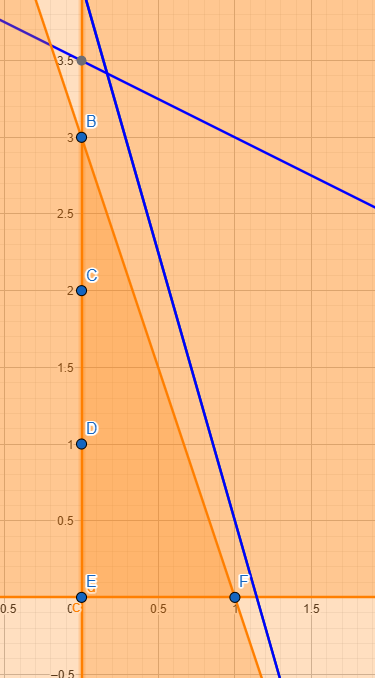
\includegraphics[width=0.5\linewidth]{img/ejercicios/Capitulo-5/ejercicio_5_4_envoltura_convexa.png}
    \caption{Envolvente convexa}
    \label{ex:5:4:fig:envoltura}
\end{figure}
  \item
Las matrices del problema relajado en formulación estándar son:
\[
A=\begin{pmatrix*}
7 & 2 & 1 & 0\\
1 & 2 & 0 & 1
\end{pmatrix*},\qquad
b=\begin{pmatrix}
8\\[0.3em]
7
\end{pmatrix},\qquad
B=\begin{pmatrix}
7 & 0\\
1 & 1
\end{pmatrix}
\]
El óptimo de la relajación lineal es
\[
(x_{1},x_{2},s_{1},s_{2})
=\Bigl(\tfrac{8}{7},\;0,\;0,\;\tfrac{41}{7}\Bigr),
\]
luego se realiza el corte sobre \(x_{1}\):
\begin{equation*}
x_{1}
\;+\;\bigl\lfloor\overline{a}_{12}\bigr\rfloor\,x_{2}
\;+\;\bigl\lfloor\overline{a}_{13}\bigr\rfloor\,s_{1}
\;\le\;\bigl\lfloor\overline{a}_{10}\bigr\rfloor
\end{equation*}
donde
\begin{align*}
\overline{a}_{12}
&=\Bigl(B^{-1}\begin{pmatrix}2\\2\end{pmatrix}\Bigr)_{1}
=\frac{2}{7},\\
\overline{a}_{13}
&=\Bigl(B^{-1}\begin{pmatrix}1\\0\end{pmatrix}\Bigr)_{1}
=\frac{1}{7},\\
\overline{a}_{10}
&=\Bigl(B^{-1}b\Bigr)_{1}
=\frac{8}{7}.
\end{align*}
De modo que el nuevo corte es:
\begin{equation*}
x_{1}\;\le\;1.
\end{equation*}
Añadiendo \(x_{1}\le1\) a la relajación original, el nuevo óptimo es
\[
(x_{1},x_{2}) = (1,0),\qquad z = -3,
\]
que ya es entero y coincide con la solución óptima del programa entero. 
\end{enumerate}
}


\subsubsection{Resolución 5.5}
% Fuente: Pauta del Control 2, Pregunta 1.
\begin{enumerate}
  \item[(a)]
 
\[
\max\; z = 5x_1+4x_2 \qquad
\text{s.a.}\quad
\begin{cases}
6x_1+4x_2 \le 24 & \text{(protecciones)}\\
x_1+2x_2 \le 6 & \text{(tablero)}\\
x_1,x_2 \ge 0,\ \text{enteros.}
\end{cases}
\]
 
\textbf{Relajaci\'on lineal.} Quitando la integralidad, los v\'ertices de la regi\'on factible son
\begin{equation}
    (0,0),\:(4,0),\:(0,3)
\end{equation}
y la intersecci\'on de ambas restricciones. Resolviendo
$6x_1+4x_2=24$ con $x_1+2x_2=6$ se obtiene $x_2=\tfrac32,\ x_1=3$. Evaluando $z$:
\[
(4,0)\to 20,\quad (0,3)\to 12,\quad \Big(3,\tfrac32\Big)\to 21.
\]
El \'optimo de la relajaci\'on es $\big(3,\tfrac32\big)$ con $\boxed{z^*_{LP}=21}$ (fraccionario en $x_2$).
 
\textbf{Envoltura convexa.} El cierre convexo de los puntos enteros factibles tiene v\'ertices
$(0,0),(4,0),(2,2),(0,3)$, basta con añadir la recta $x_1+x_2\le 4$:

\begin{center}
\begin{tikzpicture}[scale=1.35]
  \fill[gray!16]  (0,0) -- (4,0) -- (3,1.5) -- (0,3) -- cycle;
  \fill[blue!14]  (0,0) -- (4,0) -- (2,2)   -- (0,3) -- cycle;
  \draw[step=1,gray!30,very thin] (0,0) grid (4.5,3.5);
  \draw[->] (0,0) -- (4.9,0) node[right]{$x_1$};
  \draw[->] (0,0) -- (0,3.8) node[above]{$x_2$};
  \foreach \x in {1,2,3,4} \draw (\x,0.04)--(\x,-0.04) node[below]{\footnotesize\x};
  \foreach \y in {1,2,3} \draw (0.04,\y)--(-0.04,\y) node[left]{\footnotesize\y};
  % restricciones
  \draw[orange!75!black,thick] (4,0) -- (1.667,3.5) node[pos=0.85,left]{\footnotesize $6x_1{+}4x_2\le24$};
  \draw[teal!70!black,thick]   (0,3) -- (4.5,0.75) node[pos=0.92,below]{\footnotesize $x_1{+}2x_2\le6$};
  % faceta entera
  \draw[blue!70!black,very thick] (4,0) -- (2,2) node[midway,below left,blue!60!black]{\footnotesize $x_1{+}x_2\le4$};
  % puntos enteros
  \foreach \p in {(0,0),(1,0),(2,0),(3,0),(4,0),(0,1),(1,1),(2,1),(3,1),(0,2),(1,2),(2,2),(0,3)}
    \fill \p circle (1.5pt);
  % optimo relajacion
  \draw[red!75!black,thick] (3,1.5) circle (3.2pt);
  \node[red!70!black,above right,inner sep=1pt] at (3,1.5) {\footnotesize $(3,\tfrac32)$, $z{=}21$};
  % optimo entero
  \fill[green!55!black] (4,0) circle[radius=2.2pt];
  \node[green!45!black,above right,inner sep=1pt] at (4,0.05) {\footnotesize $(4,0)$, $z{=}20$};
\end{tikzpicture}
\end{center}
 
  \item[(b)]
 
Basta a\~nadir la recta añadida en la envoltura convexa
\[
\boxed{x_1+x_2 \le 4.}
\]
Con ella, la regi\'on de la relajaci\'on pasa a ser exactamente $\operatorname{conv}$, con v\'ertices
\begin{equation*}
    (0,0),\:(4,0),\:(2,2),\:(0,3) \: \implies \:\textit{todos enteros}
\end{equation*}
. La restricci\'on de potencia
$6x_1+4x_2\le24$ queda redundante (solo toca en $(4,0)$). Optimizando $z=5x_1+4x_2$:
\[
(4,0)\to 20,\quad (2,2)\to 18,\quad (0,3)\to 12 \;\Rightarrow\; \text{\'optimo LP en }(4,0),\ z=20,
\]
que coincide con el \'optimo entero. Es el corte ``ideal'': uno solo basta para obtener la solución óptima entera resolviendo el problema relajado.
 
  \item[(c)]

Aplicando el corte de Gomory sobre la fila asociada a \(x_2\),
\[
x_{B_r}+
\sum_{j\in N}
\left\lfloor (B^{-1}A_j)_r\right\rfloor x_j
\leq
\left\lfloor (B^{-1}b)_r\right\rfloor,
\qquad r=2,
\]
resulta
\[
x_2+
\left\lfloor-\frac18\right\rfloor s_1+
\left\lfloor\frac34\right\rfloor s_2
\leq
\left\lfloor\frac32\right\rfloor.
\]

Por tanto,
\[
x_2-s_1\leq 1.
\]

Usando
\[
s_1=24-6x_1-4x_2,
\]
se obtiene
\[
x_2-\left(24-6x_1-4x_2\right)\leq 1,
\]
y finalmente
\[
\boxed{6x_1+5x_2\leq 25.}
\]
 
\textbf{Verificaci\'on.} En $\big(3,\tfrac32\big)$ da $25{,}5>25$ (elimina el v\'ertice fraccionario);
en todo punto entero factible se cumple $\le 25$ (no se pierde ninguna soluci\'on entera). El nuevo
\'optimo de la relajaci\'on pasa a $\big(\tfrac{10}{3},1\big)$, $z=\tfrac{62}{3}\approx 20{,}67$
(todav\'ia fraccionario: har\'ian falta m\'as cortes).

\begin{center}
\begin{tikzpicture}[
  scale=1.25,
  >=Latex,
  axis/.style={->,line width=.75pt,gray!75},
  cA/.style={orange!80!black,line width=1.05pt},
  cB/.style={teal!65!black,line width=1.05pt},
  cNew/.style={red!70!black,line width=1.2pt},
  dot/.style={circle,fill=black!62,inner sep=1.25pt},
  tag/.style={
    font=\scriptsize,
    fill=white,
    fill opacity=.94,
    text opacity=1,
    inner sep=1.4pt,
    rounded corners=1pt
  }
]

  % Puntos geométricos relevantes
  \coordinate (O) at (0,0);
  \coordinate (B) at (4,0);
  \coordinate (C) at (3,1.5);              % óptimo anterior
  \coordinate (D) at (0,3);
  \coordinate (P) at ({10/3},1);           % nuevo óptimo
  \coordinate (Q) at ({20/7},{11/7});      % intersección rojo--verde

  % Región factible final
  \fill[teal!11] (O) -- (B) -- (P) -- (Q) -- (D) -- cycle;

  % Parte de la región anterior eliminada por la nueva restricción
  \fill[red!13] (C) -- (P) -- (Q) -- cycle;

  % Cuadrícula
  \draw[step=1,gray!22,very thin] (0,0) grid (4.5,3.5);

  % Ejes
  \draw[axis] (0,0) -- (4.9,0) node[right] {$x_1$};
  \draw[axis] (0,0) -- (0,3.8) node[above] {$x_2$};

  % Marcas de los ejes
  \foreach \x in {1,2,3,4}
    \draw (\x,.045) -- (\x,-.045)
      node[below=2pt,font=\footnotesize] {\x};

  \foreach \y in {1,2,3}
    \draw (.045,\y) -- (-.045,\y)
      node[left=2pt,font=\footnotesize] {\y};

  % Restricciones originales
  \draw[cA] (4,0) -- ({5/3},3.5);
  \draw[cB] (0,3) -- (4.5,.75);

  % Nueva restricción: 6x_1 + 5x_2 <= 25
  \draw[cNew] ({25/6},0) -- (2.5,2);

  % Puntos enteros factibles
  \foreach \x/\y in {
    0/0,1/0,2/0,3/0,4/0,
    0/1,1/1,2/1,3/1,
    0/2,1/2,2/2,
    0/3
  }
    \node[dot] at (\x,\y) {};

  % Óptimo anterior, marcado de forma discreta
  \draw[gray!70,line width=.85pt]
    ($(C)+(-.10,-.10)$) -- ($(C)+(.10,.10)$);
  \draw[gray!70,line width=.85pt]
    ($(C)+(-.10,.10)$) -- ($(C)+(.10,-.10)$);

  % Nuevo óptimo
  \fill[red!70!black] (P) circle[radius=2.55pt];
  \node[tag,text=red!70!black,anchor=south west]
    at ($(P)+(.06,.10)$)
    {$\left(\frac{10}{3},1\right)$};

  % Etiquetas limpias, fuera de las intersecciones
  \node[tag,text=teal!65!black] at (1.10,.62)
    {\scriptsize región factible};

  \node[tag,text=red!70!black,anchor=west] at (2.10,2.30)
    {$6x_1+5x_2\le 25$};

\end{tikzpicture}
\end{center}

 
 
  \item[(d)]
 
Ra\'iz: relajaci\'on $\big(3,\tfrac32\big)$, $z=21$. Se ramifica sobre la variable fraccionaria $x_2$.
La b\'usqueda en amplitud procesa por niveles: ra\'iz $\to\{x_2\le1,\ x_2\ge2\}\to\{x_1\le3,\ x_1\ge4\}$.
 
\begin{center}
\begin{tikzpicture}[
  box/.style={draw,rounded corners,align=center,minimum width=2.9cm,minimum height=1.05cm,
              font=\footnotesize,inner sep=2pt},
  opt/.style={box,very thick,fill=green!12},
  leaf/.style={box,fill=blue!6},
  edgelbl/.style={font=\scriptsize,fill=white,inner sep=1pt}
]
  \node[box]  (root) at (0,0)   {$(3,\tfrac32)$\\ $z=21$ (fracc.)};
  \node[box]  (n1)   at (-3,-2) {$(\tfrac{10}{3},1)$\\ $z\approx20{,}7$ (fracc.)};
  \node[leaf] (n2)   at (3,-2)  {$(2,2)$\\ $z=18$ (hoja)};
  \node[leaf] (n11)  at (-5,-4) {$(3,1)$\\ $z=19$ (hoja)};
  \node[opt]  (n12)  at (-1,-4) {$(4,0)$\\ $z=20$ ($\bigstar$ \'optimo)};
  \draw[->] (root) -- (n1)  node[edgelbl,pos=0.5]{$x_2\le1$};
  \draw[->] (root) -- (n2)  node[edgelbl,pos=0.5]{$x_2\ge2$};
  \draw[->] (n1)   -- (n11) node[edgelbl,pos=0.5]{$x_1\le3$};
  \draw[->] (n1)   -- (n12) node[edgelbl,pos=0.5]{$x_1\ge4$};
\end{tikzpicture}
\end{center}
 
\noindent\textbf{Recorrido.}
\begin{itemize}[nosep]
  \item $x_2\le1$: LP $\to\big(\tfrac{10}{3},1\big)$, $z\approx20{,}7$; fraccionaria en $x_1\Rightarrow$ se ramifica.
  \item $x_2\le1,\ x_1\le3$: LP $\to(3,1)$, $z=19$; \textbf{hoja} (entera). Incumbente provisional.
  \item $x_2\le1,\ x_1\ge4$: LP $\to(4,0)$, $z=20$; \textbf{hoja} (entera). Mejora el incumbente.
  \item $x_2\ge2$: LP $\to(2,2)$, $z=18$; \textbf{hoja} (entera), dominada por $(4,0)$.
\end{itemize}
 
\noindent Cada hoja se cierra porque su relajaci\'on ya es entera (criterio de integralidad), as\'i que
no queda nada que ramificar. El \'optimo entero es $\boxed{(x_1,x_2)=(4,0),\ z^*=20}$: instalar
$4$ m\'odulos PV y $0$ bater\'ias, abasteciendo $20$ viviendas.
 
  \item[(e)]
 
Con b\'usqueda en amplitud, los tres problemas resueltos son la \textbf{ra\'iz}, el nodo
\textbf{$x_2\le1$} y el nodo \textbf{$x_2\ge2$}. Al terminar de procesarlos:
\begin{itemize}[nosep]
  \item Incumbente (mejor entera): $(2,2)$, $\;z_{LB}=18$.
  \item Mejor cota superior de los nodos pendientes (los hijos de $x_2\le1$, a\'un sin resolver,
        que heredan la cota de su padre): $z_{UB}=\tfrac{62}{3}\approx 20{,}67$.
\end{itemize}
El gap en ese punto es
\[
\text{gap}_{\text{abs}} = z_{UB}-z_{LB} = \tfrac{62}{3}-18 = \tfrac{8}{3}\approx 2{,}67.
\]
Para que el algoritmo se detenga \emph{sin} resolver esos hijos, la tolerancia debe cumplir
\[
\boxed{\varepsilon_{\text{abs}} \ge \tfrac{8}{3}\approx 2{,}67}
\qquad\Longleftrightarrow\qquad
\varepsilon_{\text{rel}} \ge \frac{8/3}{18} = \frac{4}{27}\approx 14{,}8\%
\ \ \text{(respecto al incumbente),}
\]
o bien $\dfrac{8/3}{62/3}=\dfrac{4}{31}\approx 12{,}9\%$ respecto a la cota. Con esa tolerancia, B\&B
devuelve $(2,2)$ con $z=18$, garantizado a lo sumo $\tfrac{8}{3}$ por debajo del \'optimo (el \'optimo
real es $20$; el error real es $2$). Es el clásico compromiso entre tolerancia y esfuerzo: un gap m\'as
holgado detiene antes la b\'usqueda pero entrega una soluci\'on sub\'optima.
\end{enumerate}


\subsubsection{Resolución 5.6}
% Fuente: Pauta del Control 2, Pregunta 3, ítems 3–4.
{\color{MidnightBlue}
\begin{enumerate}
    \item \textbf{Falsa.} En un programa lineal \emph{entero}, el segmento entre dos soluciones enteras factibles no tiene por qué estar compuesto por puntos enteros.

    Por ejemplo, considérese
    \[
        \min \; 0
    \]
    sujeto a
    \[
        0\leq x\leq 1,
        \qquad x\in\mathbb{Z}.
    \]
    Las únicas soluciones factibles son $x=0$ y $x=1$. Ambas son óptimas, pues la función objetivo vale $0$ en ambas, pero no existen infinitas soluciones óptimas enteras. Por tanto, la afirmación es falsa.

    \item \textbf{Verdadera.} Sea $X_I$ la región factible del programa lineal entero. Como $P_1$ y $P_2$ son relajaciones del problema entero, se cumple
    \[
        X_I\subseteq P_1,
        \qquad
        X_I\subseteq P_2.
    \]
    En particular, como $x^*\in X_I$, entonces $x^*\in P_1$. Por consiguiente,
    \[
        c^\top x^*\geq \min_{x\in P_1} c^\top x.
    \]
    Además, dado que $P_1\subseteq P_2$, al minimizar sobre un conjunto más grande el valor óptimo no puede aumentar; así,
    \[
        \min_{x\in P_1}c^\top x
        \geq
        \min_{x\in P_2}c^\top x.
    \]
    Por tanto,
    \[
        c^\top x^*
        \geq
        \min_{x\in P_1}c^\top x
        \geq
        \min_{x\in P_2}c^\top x.
    \]
\end{enumerate}
}

